%%%%%%%% ICML 2021 EXAMPLE LATEX SUBMISSION FILE %%%%%%%%%%%%%%%%%

\documentclass{article}

% Recommended, but optional, packages for figures and better typesetting:
\usepackage{microtype}
\usepackage{graphicx}

\usepackage{subfigure}
\usepackage{booktabs} % for professional tables

% hyperref makes hyperlinks in the resulting PDF.
% If your build breaks (sometimes temporarily if a hyperlink spans a page)
% please comment out the following usepackage line and replace
% \usepackage{icml2021} with \usepackage[nohyperref]{icml2021} above.
\usepackage{hyperref}

% Attempt to make hyperref and algorithmic work together better:
\newcommand{\theHalgorithm}{\arabic{algorithm}}

% Use the following line for the initial blind version submitted for review:
% \usepackage{icml2021}

% If accepted, instead use the following line for the camera-ready submission:
\usepackage[accepted]{icml2021}

% \usepackage[
% backend=biber,
% style=numeric,
% ]{biblatex}
% \title{A bibLaTeX example}
% \addbibresource{main.bib} %Imports bibliography file


% The \icmltitle you define below is probably too long as a header.
% Therefore, a short form for the running title is supplied here:
\icmltitlerunning{3D Similarity for CAD Designs}

\begin{document}

\twocolumn[
\icmltitle{3D Similarity for CAD Designs}

% It is OKAY to include author information, even for blind
% submissions: the style file will automatically remove it for you
% unless you've provided the [accepted] option to the icml2021
% package.

% List of affiliations: The first argument should be a (short)
% identifier you will use later to specify author affiliations
% Academic affiliations should list Department, University, City, Region, Country
% Industry affiliations should list Company, City, Region, Country

% You can specify symbols, otherwise they are numbered in order.
% Ideally, you should not use this facility. Affiliations will be numbered
% in order of appearance and this is the preferred way.
\icmlsetsymbol{equal}{*}

\begin{icmlauthorlist}
\icmlauthor{Martin ACCOU}{}
\end{icmlauthorlist}

% \icmlcorrespondingauthor{Martin ACCOU}{martin.accou@icloud.com}

% You may provide any keywords that you
% find helpful for describing your paper; these are used to populate
% the "keywords" metadata in the PDF but will not be shown in the document
\icmlkeywords{Machine Learning, ICML}

\vskip 0.3in
]

% this must go after the closing bracket ] following \twocolumn[ ...

% This command actually creates the footnote in the first column
% listing the affiliations and the copyright notice.
% The command takes one argument, which is text to display at the start of the footnote.
% The \icmlEqualContribution command is standard text for equal contribution.
% Remove it (just {}) if you do not need this facility.

% \printAffiliationsAndNotice{}  % leave blank if no need to mention equal contribution
% \printAffiliationsAndNotice{\icmlEqualContribution} % otherwise use the standard text.

\begin{abstract}
This research addresses the challenge of managing large, poorly labeled 3D CAD design repositories in industrial settings. We present a novel approach to developing a 3D similarity model using a combination of innovative triplet generation techniques, a user-friendly labeling application, and state-of-the-art deep learning models. Our method employs self-supervised learning with contrastive techniques to overcome the limitation of sparse labeled data. We developed a 'Tinder-like' application for efficient human labeling of design triplets and implemented an iterative process of model training and triplet generation. Experiments were conducted using both Graph Neural Network (GNN) and Transformer-based architectures, with the latter, specifically the OpenShape encoder, demonstrating superior performance in terms of accuracy, rotation invariance, and qualitative assessments. The resulting model shows promise in automating design comparison and retrieval, potentially transforming how engineers interact with vast design databases. Future work includes exploring multi-modal similarity models and implementing active learning strategies for more efficient triplet selection. This approach offers significant potential for enhancing design reuse and information retrieval in industrial CAD applications.
\end{abstract}

\section{Introduction}
\label{intro}

D3S, a leader in 3D CAD Analytics and NLP, develops AI-powered solutions for industries like aerospace and automotive. Their current focus is on \textbf{creating a 3D similarity model to compare CAD designs based solely on geometric properties} (\autoref{fig:purpose}). This innovation addresses significant challenges in managing large CAD repositories, where inefficient design retrieval leads to time wastage, duplicated efforts, and missed opportunities for innovation.

\begin{figure}[h]
    \centering
    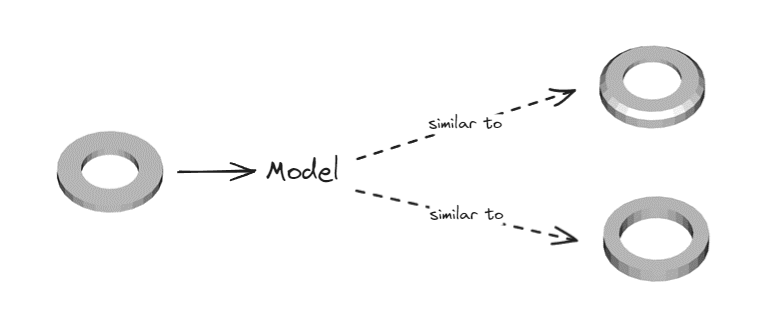
\includegraphics[width=0.8\columnwidth]{assets/similar-pieces.png}
    \caption{Purpose of the 3D similarity model.}
    \label{fig:purpose}
\end{figure}
Traditional manual classification methods have proven inconsistent and unscalable, prompting the need for an automated solution. The proposed 3D similarity model aims to streamline design comparison and retrieval, potentially transforming how engineers interact with vast design databases.
Faced with limited labeled data, we adopted a self-supervised learning approach using contrastive learning. We developed a novel 'Tinder-like' application to build a labeled triplets database.

The project pipeline involves two main steps: \textbf{triplet collection through this app}, and \textbf{model training to compute similarities between 3D designs}.

\section{Method}

The proposed method for constructing a similarity model from an unlabeled dataset with a small proportion of labeled instances is generalizable beyond 3D CAD designs. The process involves generating unlabeled triplets, labeling them through a dedicated application, and training a model using triplet loss.

\textbf{A key component is the user-friendly labeling application}, which serves two main purposes: labeling triplets and comparing model iterations. For labeling, users are presented with three 3D designs and must choose which is more similar to the central anchor design, as shown in \autoref{fig:labeling}. The app includes features like canonical view options and additional metadata to aid decision-making.

\begin{figure}[h]
    \centering
    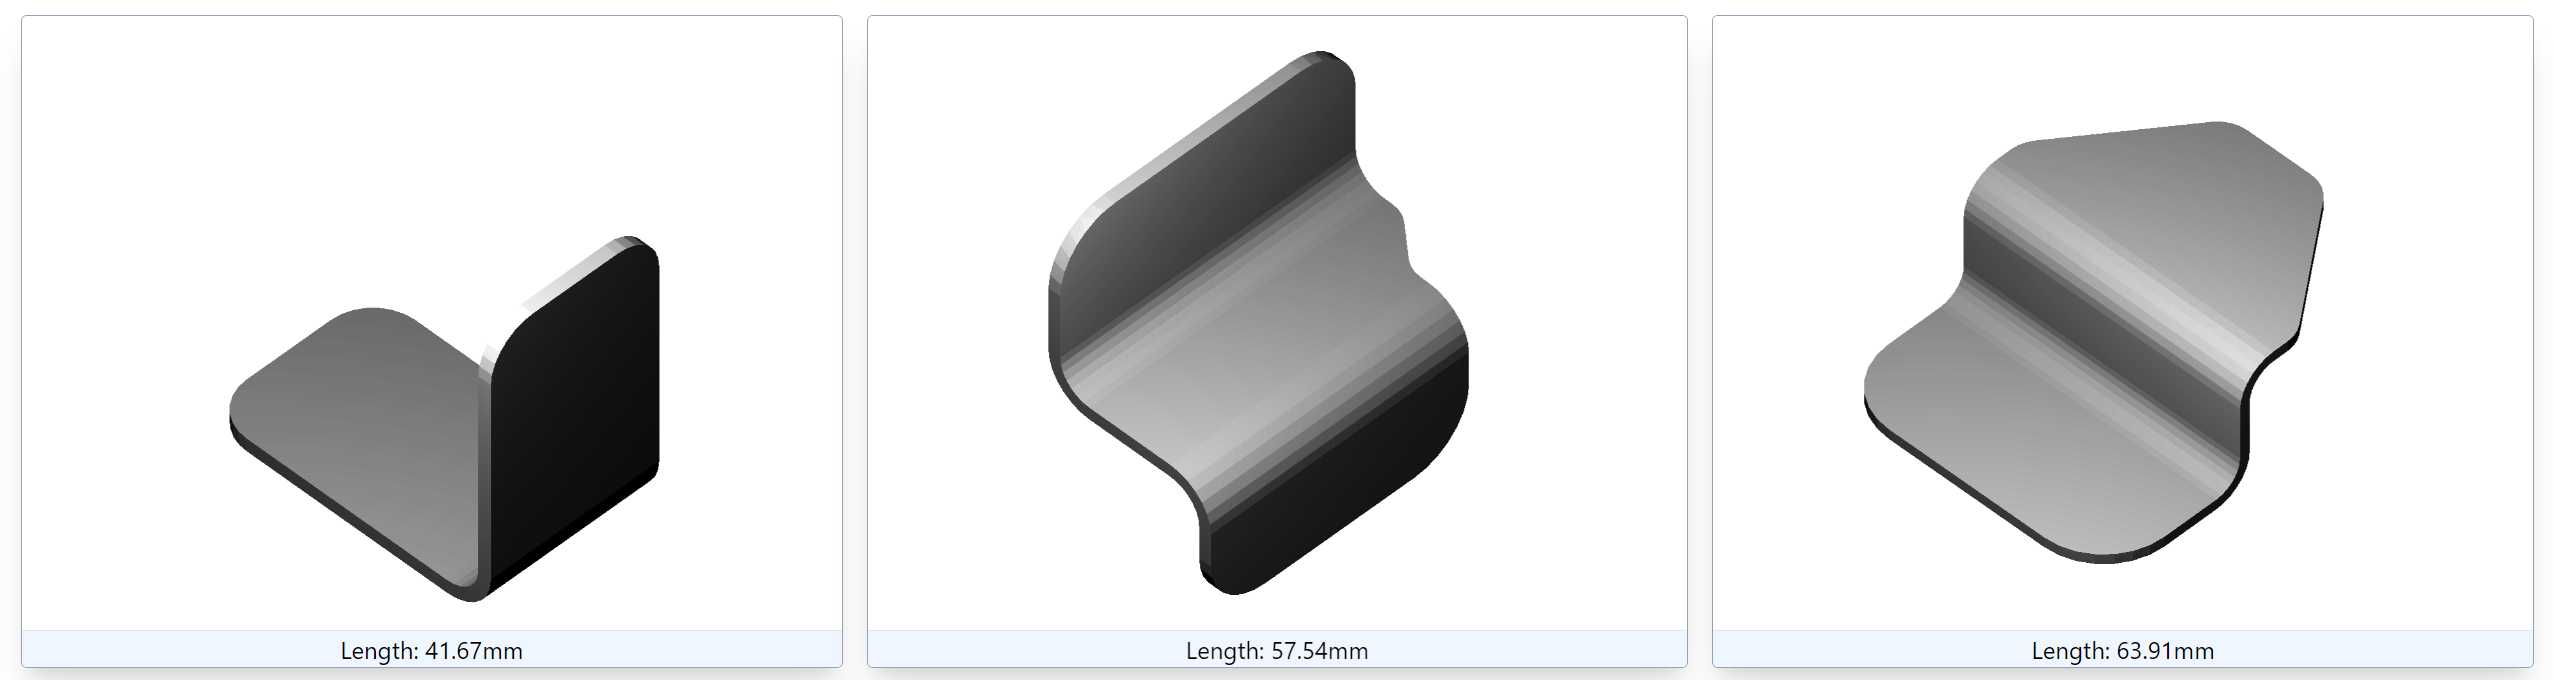
\includegraphics[width=\columnwidth]{assets/tinder3d_labeling.png}
    \caption{User interface for the labeling use case. Here, the design on the right is more similar to the anchor design in the center.}
    \label{fig:labeling}
\end{figure}

The triplet loss training aims to create a representation where similar instances are close together and dissimilar ones are far apart in the embedding space. The loss function is designed to handle easy, hard, and semi-hard triplets, with the balance between these types crucial for model performance.

Triplet generation is an iterative process, starting with a model trained on a small labeled dataset and refining it through subsequent labeling rounds. The goal is to generate diverse, labelable triplets that challenge the model, striking a balance between user experience and model improvement.

This method has shown promising results, achieving accuracy comparable to classification models with relatively few labeled triplets. It offers a practical approach to building effective similarity models in domains with limited labeled data.


\section{Experiments}

The experiments for the 3D similarity model were conducted using a dataset of 20,000 triplets, with consistent training configurations across two main model architectures: Graph Neural Networks (GNN) and Transformer-based models.

Data preparation involved converting meshes to graphs for the GNN model and to point clouds for the Transformer model. Data augmentation techniques, particularly random rotations and normalization to unit sphere, were employed to enhance model robustness and rotation invariance. Offline augmentation proved more effective than online augmentation.
Several metrics were defined to evaluate model performance, including triplet order accuracy, rotation invariance measures, and test accuracy on a small labeled dataset. We also relied heavily on qualitative assessment through a user interface.

The GNN model, based on EdgeConv architecture, showed initial promise but faced challenges in maintaining performance as training progressed. Key learnings included the importance of batch normalization, large batch sizes, and careful management of triplet loss training.

The transition to Transformer-based models, particularly the OpenShape architecture, yielded significant improvements. The pre-trained model outperformed the best GNN model, and fine-tuning further enhanced results. \textbf{The Transformer model demonstrated a better ability to learn correct triplet ordering and improve rotation invariance metrics throughout training}.

Visualizations of the embeddings in 3D space, such as \autoref{fig:clusters}, revealed the model's capacity to cluster similar designs, even without explicit labels. However, we noted that quantitative metrics didn't always align with qualitative assessments, highlighting the importance of human evaluation in this unsupervised learning context.

\begin{figure}[h]
    \centering
    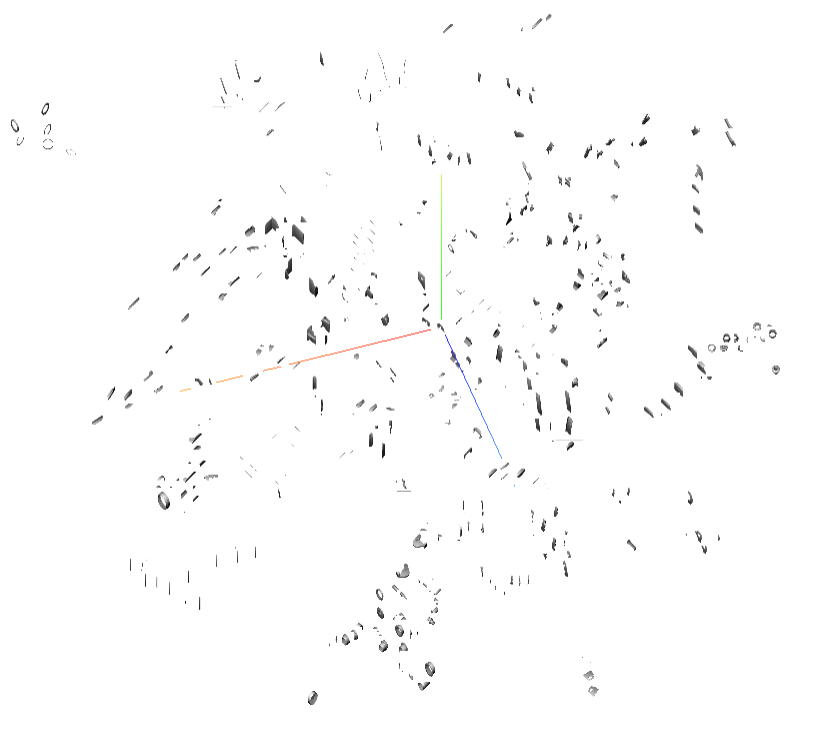
\includegraphics[width=0.7\columnwidth]{assets/clusters_tsne.png}
    \caption{t-SNE visualization of the embeddings in 3D space.}
    \label{fig:clusters}
\end{figure}

\section{Conclusion and perspectives}

This work presents a novel approach to 3D CAD design similarity in industrial settings, addressing the challenge of large, poorly labeled repositories. The developed pipeline combines innovative triplet generation, a user-friendly labeling application, and state-of-the-art deep learning models. 

Key contributions include a method for generating diverse unlabeled triplets, a "Tinder-like" application for efficient human labeling, an iterative process of model training and triplet generation, and experimentation with both graph-based and transformer-based models. The transformer-based model yielded superior results across all metrics. 

Immediate applications include automated design optimization and integration with CAD software, particularly for suggesting improvements and inferring missing information.

\textbf{A natural follow-up is to explore 3D part segmentation}, and first tries have shown promising results (\autoref{fig:seg}). 

\begin{figure}[h]
    \centering
    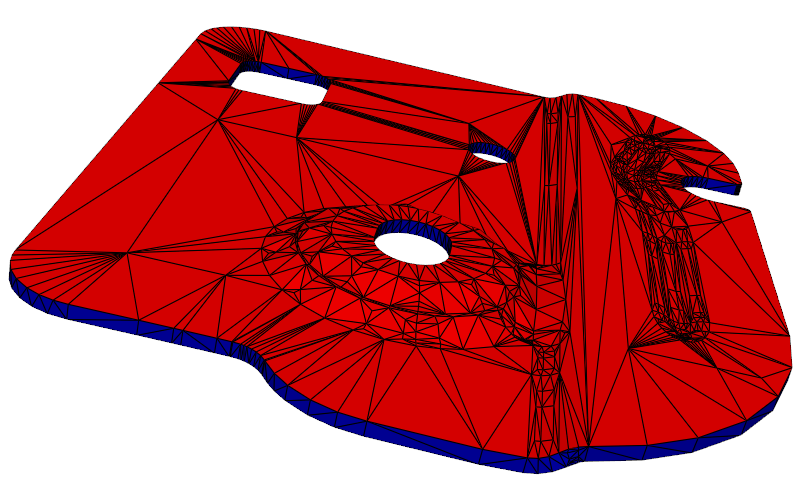
\includegraphics[width=.7\columnwidth]{assets/seg_0.png}
    \caption{Segmentation of a sheet metal design. In blue, the "deburring". In red, the "front" and the "back".}
    \label{fig:seg}
\end{figure}

% In the unusual situation where you want a paper to appear in the
% references without citing it in the main text, use \nocite
\nocite{langley00}

% \printbibliography


%%%%%%%%%%%%%%%%%%%%%%%%%%%%%%%%%%%%%%%%%%%%%%%%%%%%%%%%%%%%%%%%%%%%%%%%%%%%%%%
%%%%%%%%%%%%%%%%%%%%%%%%%%%%%%%%%%%%%%%%%%%%%%%%%%%%%%%%%%%%%%%%%%%%%%%%%%%%%%%
% DELETE THIS PART. DO NOT PLACE CONTENT AFTER THE REFERENCES!
%%%%%%%%%%%%%%%%%%%%%%%%%%%%%%%%%%%%%%%%%%%%%%%%%%%%%%%%%%%%%%%%%%%%%%%%%%%%%%%
%%%%%%%%%%%%%%%%%%%%%%%%%%%%%%%%%%%%%%%%%%%%%%%%%%%%%%%%%%%%%%%%%%%%%%%%%%%%%%%
%%%%%%%%%%%%%%%%%%%%%%%%%%%%%%%%%%%%%%%%%%%%%%%%%%%%%%%%%%%%%%%%%%%%%%%%%%%%%%%
%%%%%%%%%%%%%%%%%%%%%%%%%%%%%%%%%%%%%%%%%%%%%%%%%%%%%%%%%%%%%%%%%%%%%%%%%%%%%%%


\end{document}


% This document was modified from the file originally made available by
% Pat Langley and Andrea Danyluk for ICML-2K. This version was created
% by Iain Murray in 2018, and modified by Alexandre Bouchard in
% 2019 and 2021. Previous contributors include Dan Roy, Lise Getoor and Tobias
% Scheffer, which was slightly modified from the 2010 version by
% Thorsten Joachims & Johannes Fuernkranz, slightly modified from the
% 2009 version by Kiri Wagstaff and Sam Roweis's 2008 version, which is
% slightly modified from Prasad Tadepalli's 2007 version which is a
% lightly changed version of the previous year's version by Andrew
% Moore, which was in turn edited from those of Kristian Kersting and
% Codrina Lauth. Alex Smola contributed to the algorithmic style files.
